\documentclass{article}
\usepackage{graphicx}

\graphicspath{{./assets/}}

\title{Homework 1}
\author{Igor Alentev}

\begin{document}

\maketitle
\newpage

\section*{Problem 1}
\subsection*{Introduction}
We were required to implement control with constant velocities and check whether 
simulation leads to expected result.

\begin{enumerate}
        \item $v = 0.5\; \omega=0$
        \item $v = 1.0\; \omega=2$
        \item $v = 0.0\; \omega=2$
        \item $\omega_L = 20.0\; \omega_R=18.0$

\end{enumerate}

Parameters for simulation I have taken from the \textit{URDF} of the \textit{hagen\_gazebo} package.
I.e. $r=0.14\; L=0.035, \Delta t=0.033$. Time of simulation was $T=5$ seconds.

\subsection*{Simulation}

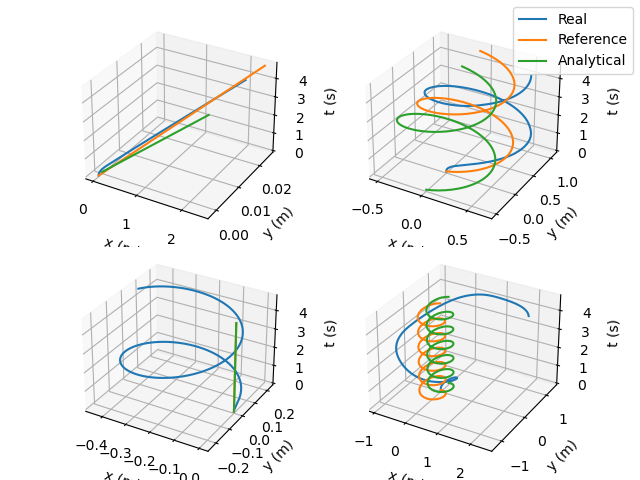
\includegraphics[scale=0.7]{3dtrajectories.png}

Here you can see three types of trajectories.

\newpage

\begin{enumerate}
    \item \textbf{Real trajectory} of the robot, streamed directly from \textbf{odometry} topic.
    \item \textbf{Reference trajectory} - expected trajectory of the robot, calculated through numerical integration on each step.
    \item \textbf{Analytical trajectory} - expected trajectory of the robot, calculated analytically.
\end{enumerate}

All of them are plotted as $(x, y)$ against time. Even though they give
pretty good visualisation of the robot motion, I would prefer their
projection on the plane, omitting evolution in time, since it is more intuitive.

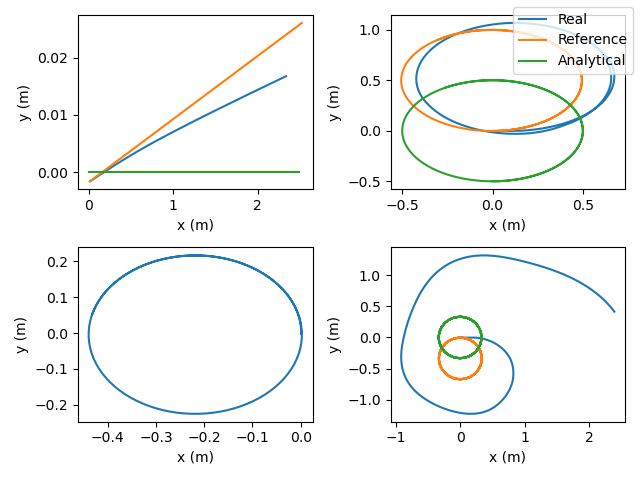
\includegraphics[scale=0.7]{trajectories.png}

\textbf{Notes:} 
\begin{itemize}
  \item First plot reference line shows exactly linear dependency, since
we have only linear component. It does not coincide with analytical solution, since
our initial angle is probably nonzero, so our straight line is not parallel to the $Ox$.
  \item On the the bottom-left plot reference and analytical solution leads to a single point at $(0, 0)$,
since parameters describe only rotation, without linear motion. However, as we can see, our robot is moving, since
due physical constraints it can not rotate without motion. On all other plots results are pretty similar and will
be considered further.
  \item I have decided not to calculate exact values of errors against time, since it is obvious
    that our oversimplified model leads to large errors and does not predict real behaviour. As a result
    I have included only plots of the trajectories and their analysis.
\end{itemize}


\subsection*{Conclusion}

First of all, as we can see, shape and parameters of the reference and analytical trajectories are completely the same.
The only difference is in initial conditions. As a result, orientation and centers of rotation slightly differ.
Similarity of these trajectories show that it is not really important which way to calculate the expected
trajectory. I would like to stick to numerical methods, since they are more flexible and intuitive.

Secondly, we can see, that the real trajectory differs a lot from the expected one. 
There are multiple reasons for this.
First of all, our analytical solutions do not consider any physical properties of the robot.
Such as dimensions of the wheels, distance between the wheels, displaced center of rotation. As a result,
our simplified model, where we consider robot as a material point simply do not reflect real behaviour.
For example, parallel placement of the wheels do not allow robot to rotate as a point would.
Moreover, distance between the wheels and rear axle plays important role as well.
even though it is a simple differential drive robot, it's rotation is not described by a simple circle.
\\\\
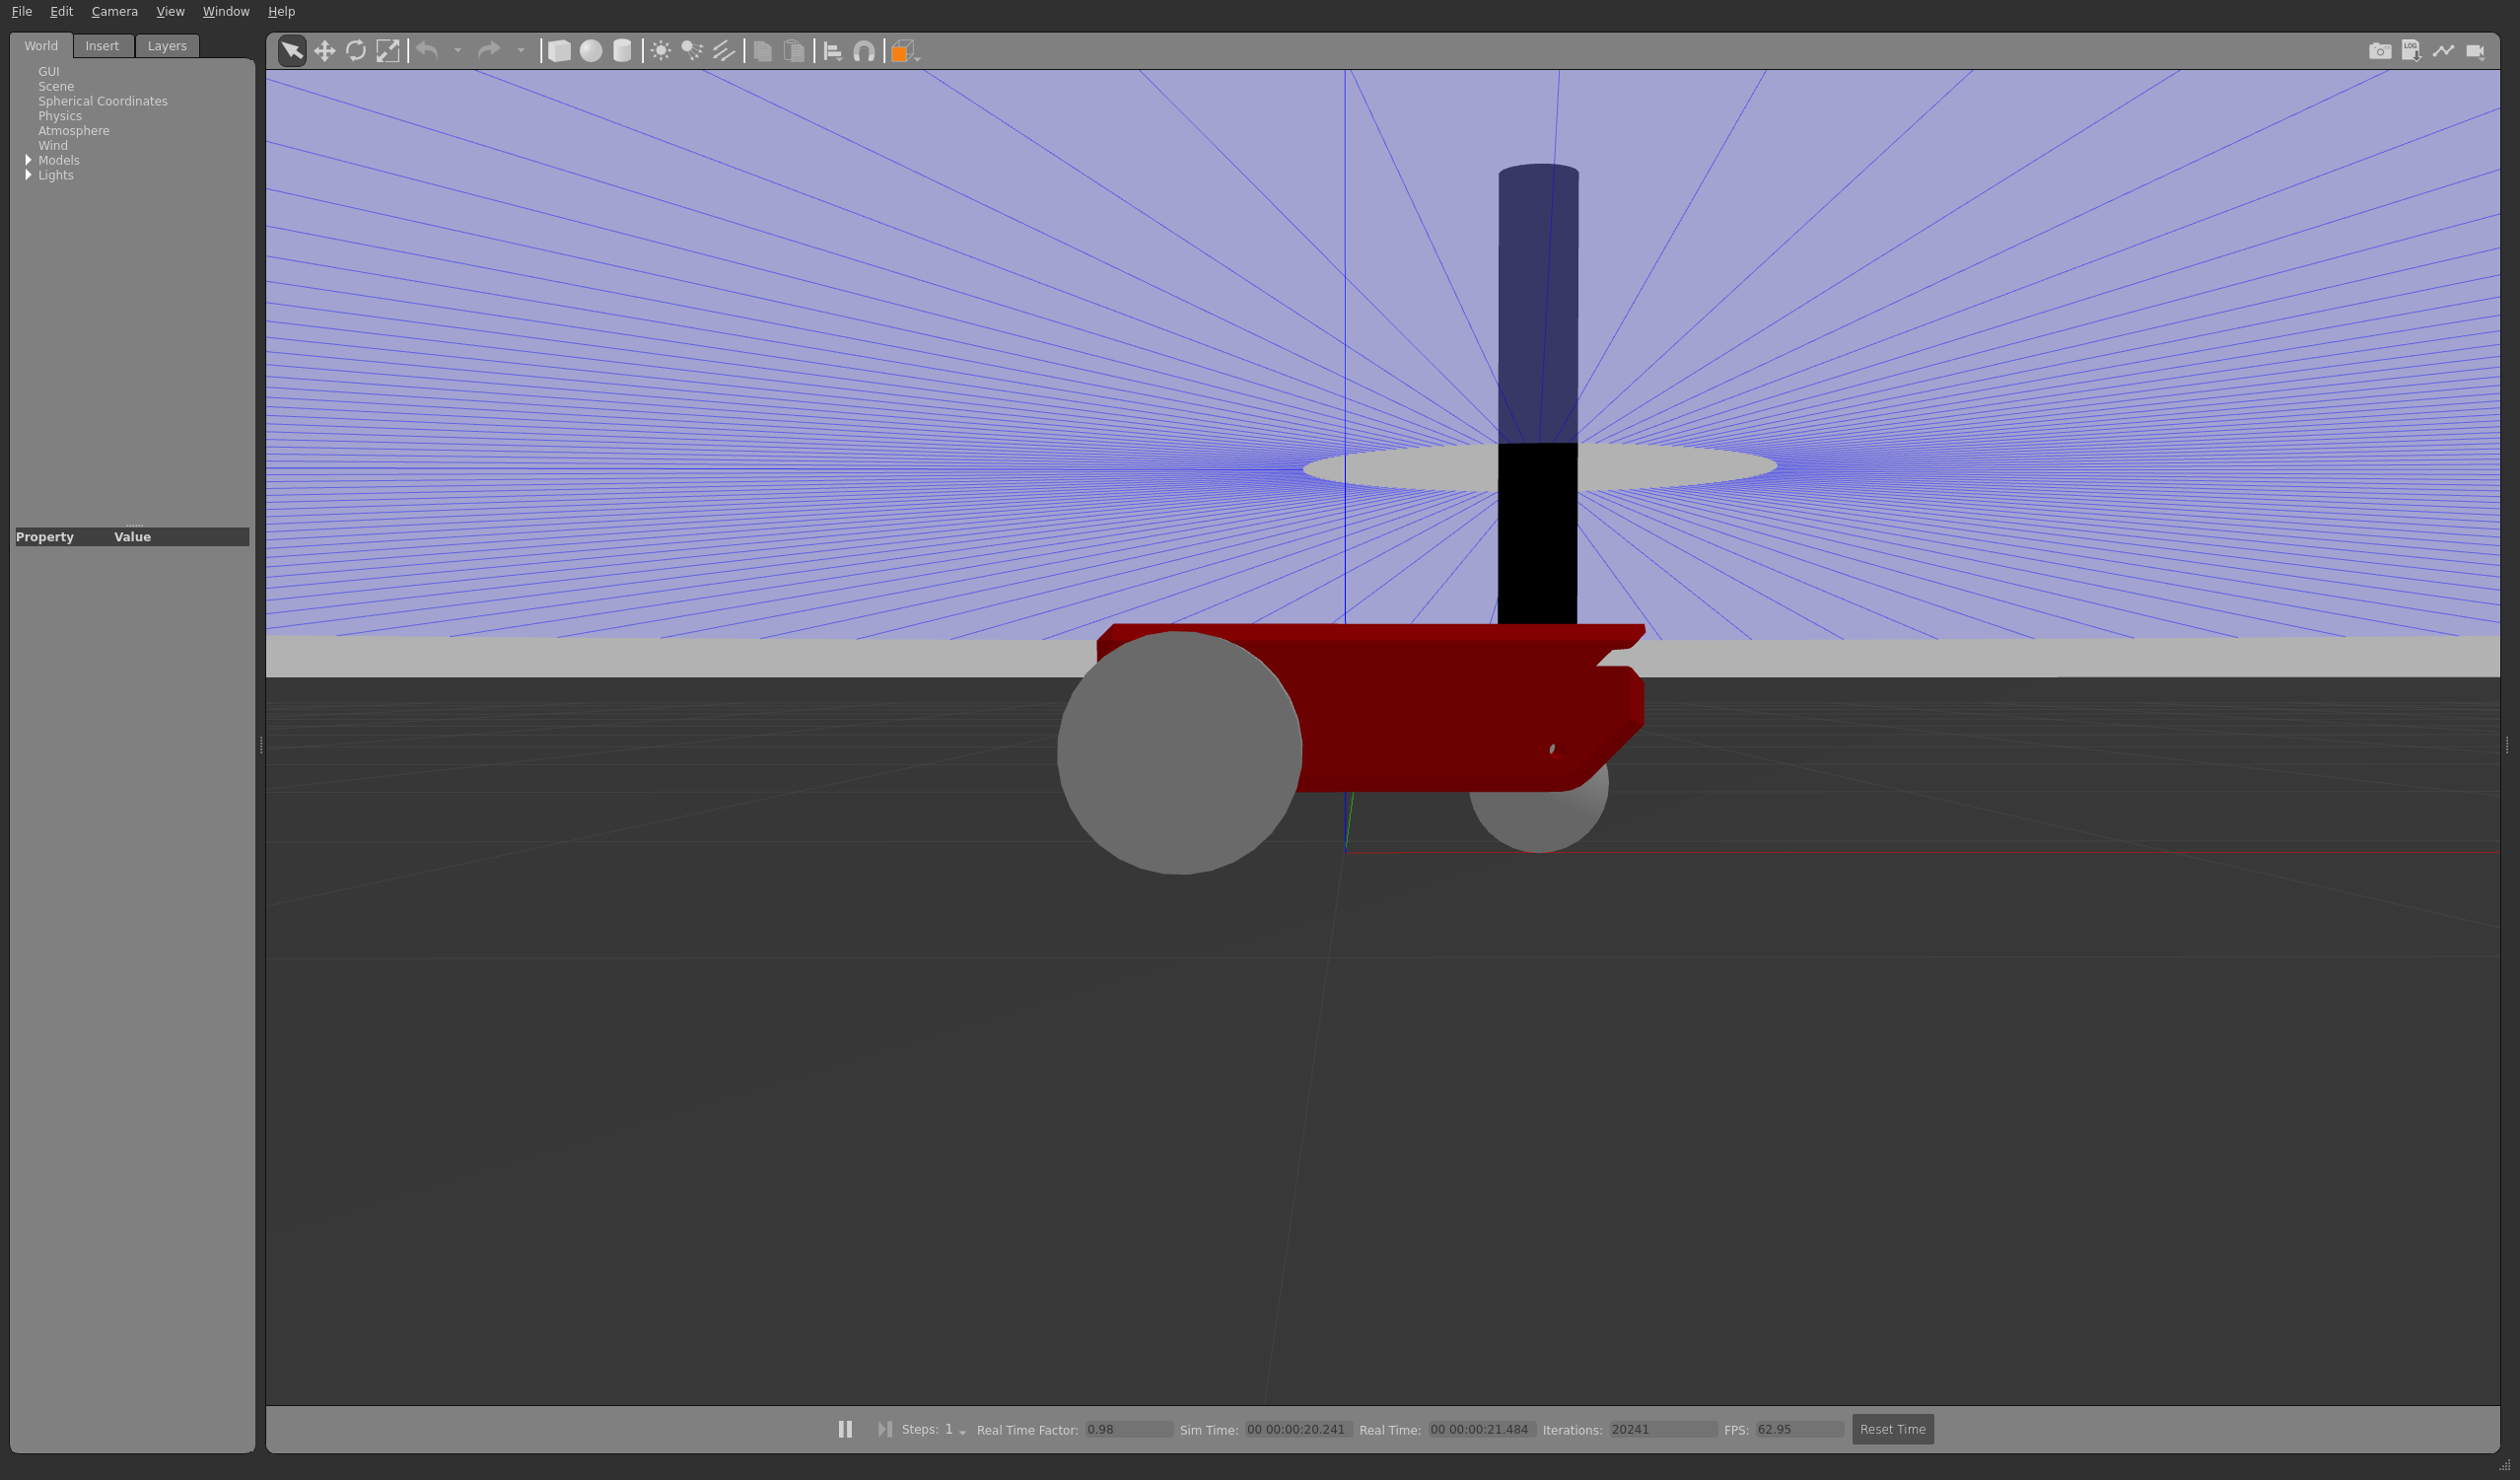
\includegraphics[scale=0.18]{assets/robot.png}

The best way to describe robot motion is to take into consideration it's physical properties. Oversimplified
dynamical model of the robot creates such large errors. If we will consider all the dimensions and stop using
material point model, we can achieve better accuracy.

The next step of improving result is reducing the sampling period. Large sampling period does not
consider errors which accumulated continouosly rather than in a discrete way. As a result, it can
lead to large divergence in results.

\end{document}
